\documentclass[a4paper,10pt]{beamer}

\usepackage{../préambule-beamer}
\usetikzlibrary{arrows.meta,positioning}

\begin{document}

\begin{frame}
	\begin{center}
		\LARGE
		\myuline{Activité : Chasse au trésor}
	\end{center}
\end{frame}

\begin{frame}
	\begin{center}
		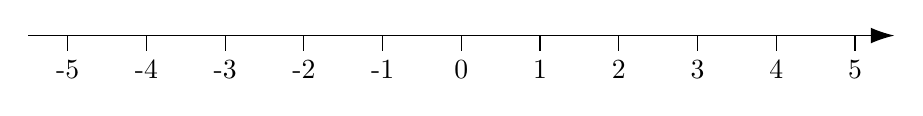
\begin{tikzpicture}
			\draw[-{Latex[length=3mm, width=2mm]}] (-5.5,0) -- (5.5,0);

			\foreach \x in {-5,...,5} {
					\draw (\x,0) -- ++(0,-0.2) node[below] {\x};
				}
		\end{tikzpicture}
	\end{center}
\end{frame}

\begin{frame}
	\begin{center}
		\begin{tikzpicture}
			\draw[-{Latex[length=3mm, width=2mm]}] (-5.5,0) -- (5.5,0);

			\foreach \x in {-5,...,5} {
					\draw (\x,0) -- ++(0,-0.2) node[below] {\x};
				}
			\node (A) at (3,0) {X};
			\node[above=of A] {A};
		\end{tikzpicture}
	\end{center}
\end{frame}

\begin{frame}
	\begin{center}
		\begin{tikzpicture}
			\draw[-{Latex[length=3mm, width=2mm]}] (-5.5,0) -- (5.5,0);

			\foreach \x in {-5,...,5} {
					\draw (\x,0) -- ++(0,-0.2) node[below] {\x};
				}
			\node (A) at (3,0) {X};
			\node[above=of A] {A};
			\node (B) at (-3,0) {X};
			\node[above=of B] {B};
		\end{tikzpicture}
	\end{center}
\end{frame}

\begin{frame}
	\begin{center}
		\begin{tikzpicture}
			\draw[-{Latex[length=3mm, width=2mm]}] (-5.5,0) -- (5.5,0);

			\foreach \x in {-5,...,5} {
					\draw (\x,0) -- ++(0,-0.2) node[below] {\x};
				}
			\node (A) at (3,0) {X};
			\node[above=of A] {A};
			\node (B) at (-3,0) {X};
			\node[above=of B] {B};
			\node (C) at (1,0) {X};
			\node[above=of C] {C};
		\end{tikzpicture}
	\end{center}
\end{frame}

\begin{frame}
	\begin{center}
		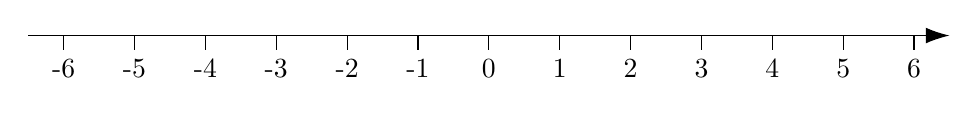
\begin{tikzpicture}[scale=0.9]
			\draw[-{Latex[length=3mm, width=2mm]}] (-6.5,0) -- (6.5,0);

			\foreach \x in {-6,...,6} {
					\draw (\x,0) -- ++(0,-0.2) node[below] {\x};
				}
		\end{tikzpicture}
	\end{center}
\end{frame}

\begin{frame}
	\begin{center}
		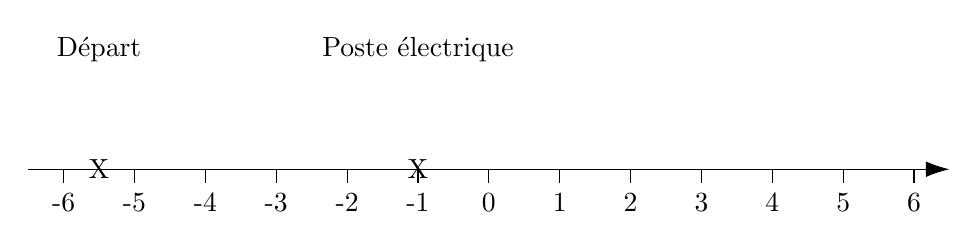
\begin{tikzpicture}[scale=0.9]
			\draw[-{Latex[length=3mm, width=2mm]}] (-6.5,0) -- (6.5,0);

			\foreach \x in {-6,...,6} {
					\draw (\x,0) -- ++(0,-0.2) node[below] {\x};
				}
			\node (depart) at (-5.5,0) {X};
			\node[above=of depart] {Départ};
			\node (poste) at (-1,0) {X};
			\node[above=of poste] {Poste électrique};
		\end{tikzpicture}
	\end{center}
\end{frame}

\begin{frame}
	\begin{center}
		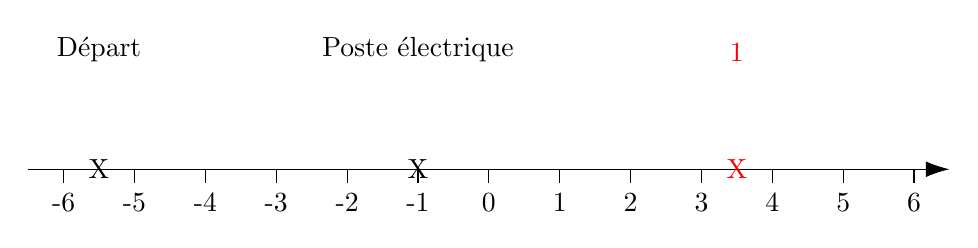
\begin{tikzpicture}[scale=0.9]
			\draw[-{Latex[length=3mm, width=2mm]}] (-6.5,0) -- (6.5,0);

			\foreach \x in {-6,...,6} {
					\draw (\x,0) -- ++(0,-0.2) node[below] {\x};
				}
			\node (depart) at (-5.5,0) {X};
			\node[above=of depart] {Départ};
			\node (poste) at (-1,0) {X};
			\node[above=of poste] {Poste électrique};
			\node[red] (A) at (3.5,0) {X};
			\node[red,above=of A] {1};
		\end{tikzpicture}
	\end{center}
\end{frame}

\begin{frame}
	\begin{center}
		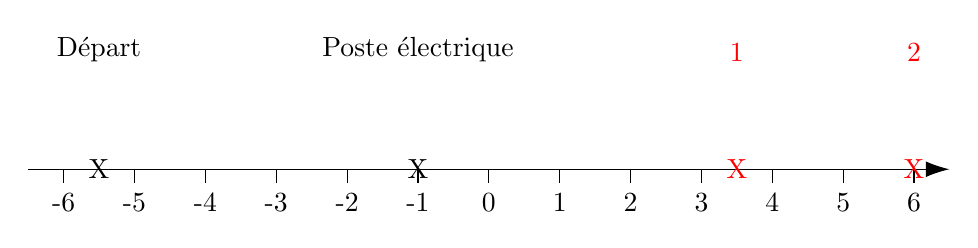
\begin{tikzpicture}[scale=0.9]
			\draw[-{Latex[length=3mm, width=2mm]}] (-6.5,0) -- (6.5,0);

			\foreach \x in {-6,...,6} {
					\draw (\x,0) -- ++(0,-0.2) node[below] {\x};
				}
			\node (depart) at (-5.5,0) {X};
			\node[above=of depart] {Départ};
			\node (poste) at (-1,0) {X};
			\node[above=of poste] {Poste électrique};
			\node[red] (A) at (3.5,0) {X};
			\node[red,above=of A] {1};
			\node[red] (B) at (6,0) {X};
			\node[red,above=of B] {2};
		\end{tikzpicture}
	\end{center}
\end{frame}

\begin{frame}
	\begin{center}
		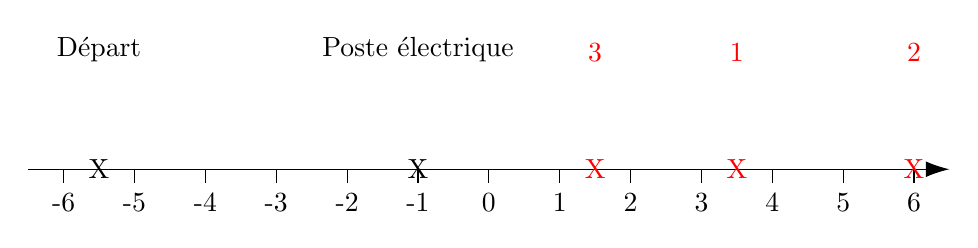
\begin{tikzpicture}[scale=0.9]
			\draw[-{Latex[length=3mm, width=2mm]}] (-6.5,0) -- (6.5,0);

			\foreach \x in {-6,...,6} {
					\draw (\x,0) -- ++(0,-0.2) node[below] {\x};
				}
			\node (depart) at (-5.5,0) {X};
			\node[above=of depart] {Départ};
			\node (poste) at (-1,0) {X};
			\node[above=of poste] {Poste électrique};
			\node[red] (A) at (3.5,0) {X};
			\node[red,above=of A] {1};
			\node[red] (B) at (6,0) {X};
			\node[red,above=of B] {2};
			\node[red] (C) at (1.5,0) {X};
			\node[red,above=of C] {3};
		\end{tikzpicture}
	\end{center}
\end{frame}

\begin{frame}
	\begin{center}
		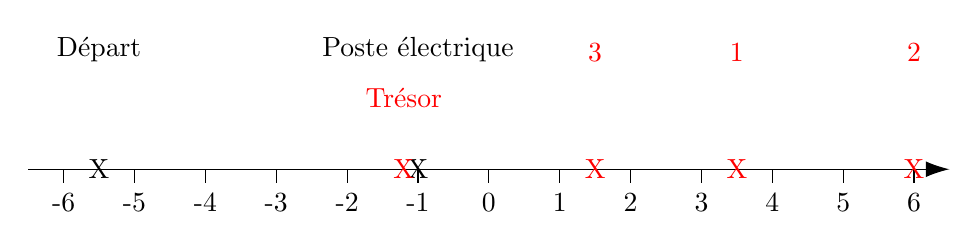
\begin{tikzpicture}[scale=0.9]
			\draw[-{Latex[length=3mm, width=2mm]}] (-6.5,0) -- (6.5,0);

			\foreach \x in {-6,...,6} {
					\draw (\x,0) -- ++(0,-0.2) node[below] {\x};
				}
			\node (depart) at (-5.5,0) {X};
			\node[above=of depart] {Départ};
			\node (poste) at (-1,0) {X};
			\node[above=of poste] {Poste électrique};
			\node[red] (A) at (3.5,0) {X};
			\node[red,above=of A] {1};
			\node[red] (B) at (6,0) {X};
			\node[red,above=of B] {2};
			\node[red] (C) at (1.5,0) {X};
			\node[red,above=of C] {3};
			\node[red] (tresor) at (-1.2,0) {X};
			\node[red] at ([yshift=1cm] tresor) {Trésor};
		\end{tikzpicture}
	\end{center}
\end{frame}


\end{document}